\chapter{Experiments}
\label{ch:experiments}

\section{Datasets}
\label{sec:ds}

In this section we consider datasets that are separated in two opposing communities. The information about the opinions of each member of this community is known. Thus, we can assign internal opinions -1 and 1 to the nodes depending on their community membership\cite{tsapMatakosTerzi}. 

\begin{enumerate}

  \item The Karate dataset, that represents the friendships between the members of a karate club at a US university. This network is split in two equal size polarized communities arround two rival instructors.
  
  \item The Books dataset that is a networkd of US politics books. These books were published near the 2004 presidential election and sold by Amazon.com . These Books are classified as "Liberal", "Conservative", or "Neutral".
  
  \item The Blogs dataset. A network of hyperlinks between online blogs on US politics.
  
\end{enumerate}
\section{Experiments with heuristics}
\label{sec:experimHeuristics}

 We evaluate the heuristic algorithms by comparing them with the naive. The goal is to validate that they minimize the polarization index in the same way the naive algorithm does but in less time. 


\begin{table}[htbp]
 \centering
 \caption{Heuristics algorithms comparison on the Karate}
 \label{tab:heuristicsKarate}
 \begin{tabular}{|c |l| c | c | c | c ||}
 \hline
  Algorithm & $\pi(z)$ Before &  $\pi(z)$ After & Time (sec) & k\\
  \hline
  \hline
  Naive  & $0.35857$ & 0.23116 &  0.71483&5 \\
  \hline
  Merge & $0.35857$ & 0.23979 &  0.04088&5 \\
  \hline
  Distance &  $0.35857$ & 0.31491 &  0.00237 &5\\
  \hline
  \hline
  Naive &  $0.35857$ & 0.19331 &  0.54732 &10\\
  \hline
  Merge &  $0.35857$ & 0.18291 &  0.05307&10 \\
  \hline
  Distance &  $0.35857$ & 0.29321 &  0.00436&10\\
  \hline
  \hline
  Naive &  $0.35857$ & 0.17656 &  0.55274 &15\\
  \hline
  Merge &  $0.35857$ & 0.16946 &  0.04806&15\\
  \hline
  Distance &  $0.35857$ & 0.28158 &  0.00515&15\\
  \hline
  \hline
  Naive &  $0.35857$ & 0.14977 &  0.5511 &20\\
  \hline
  Merge &  $0.35857$ & 0.14569 &  0.05337&20\\
  \hline
  Distance &  $0.35857$ & 0.24387 &  0.00671&20\\
  \hline
 \end{tabular}
\end{table}

\begin{figure}[!htbp]
	\centering
	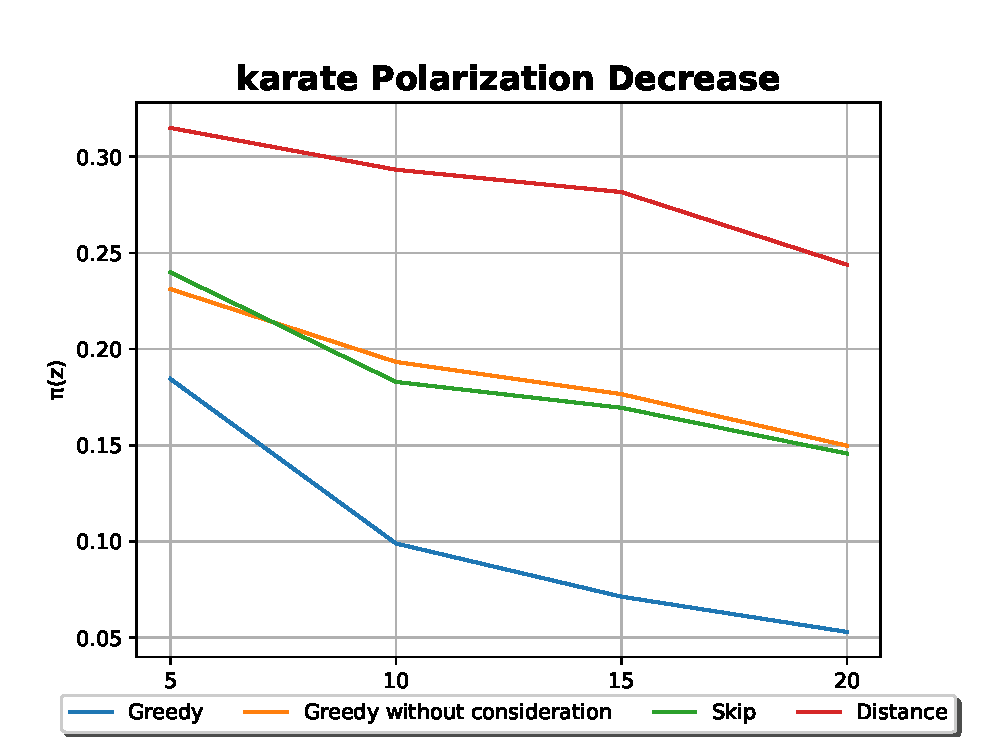
\includegraphics[width=0.65\textwidth]{Figures/karate_pol}
	\caption{Heuristic comparison of the decrease in Karate}
	\label{fig:karate_pol}
\end{figure}


\begin{figure}[!htbp]
	\centering
	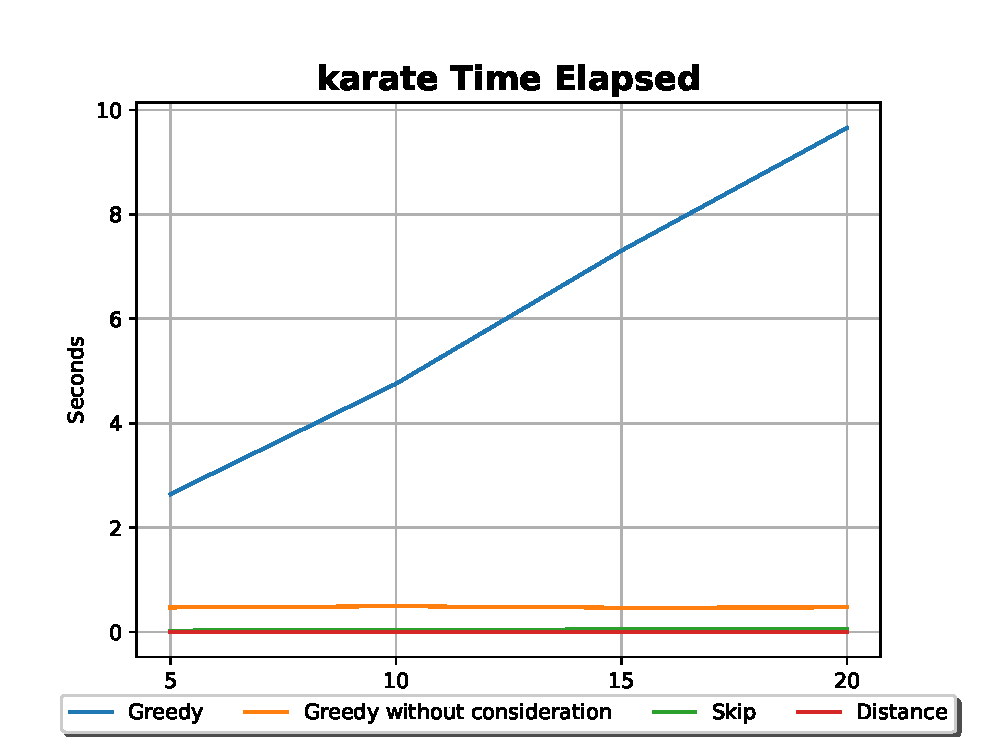
\includegraphics[width=0.65\textwidth]{Figures/karate_time}
	\caption{Heuristic comparison of time in Karate}
	\label{fig:karate_time}
\end{figure}

\begin{table}[htbp]
 \centering
 \caption{Heuristics algorithms comparison on the Books}
 \label{tab:heuristicsKarate}
 \begin{tabular}{|c |l| c | c | c | c ||}
 \hline
  Algorithm & $\pi(z)$ Before &  $\pi(z)$ After & Time (sec) & k\\
  \hline
  \hline
  Naive  & $0.44046$ & 0.35138 &  28.76573&5 \\
  \hline
  Merge & $0.44046$ & 0.43515 &  0.3107&5 \\
  \hline
  Distance &  $0.44046$ & 0.43547 &  0.01219 &5\\
  \hline
  \hline
  Naive &  $0.44046$ & 0.30969 &  28.13354 &10\\
  \hline
  Merge &  $0.44046$ & 0.43006 &  0.32842&10 \\
  \hline
  Distance &  $0.44046$ & 0.41711 &  0.01954&10\\
  \hline
  \hline
  Naive &  $0.44046$ & 0.28730 &  26.88918 &15\\
  \hline
  Merge &  $0.44046$ & 0.39831 &  0.34483&15\\
  \hline
  Distance &  $0.44046$ & 0.39297 &  0.02893&15\\
  \hline
  \hline
  Naive &  $0.44046$ & 0.26987 &  29.96203 &20\\
  \hline
  Merge &  $0.44046$ & 0.36770 &  0.37486&20\\
  \hline
  Distance &  $0.44046$ & 0.38424 &  0.03249&20\\
  \hline
 \end{tabular}
\end{table}

\begin{figure}[!htbp]
	\centering
	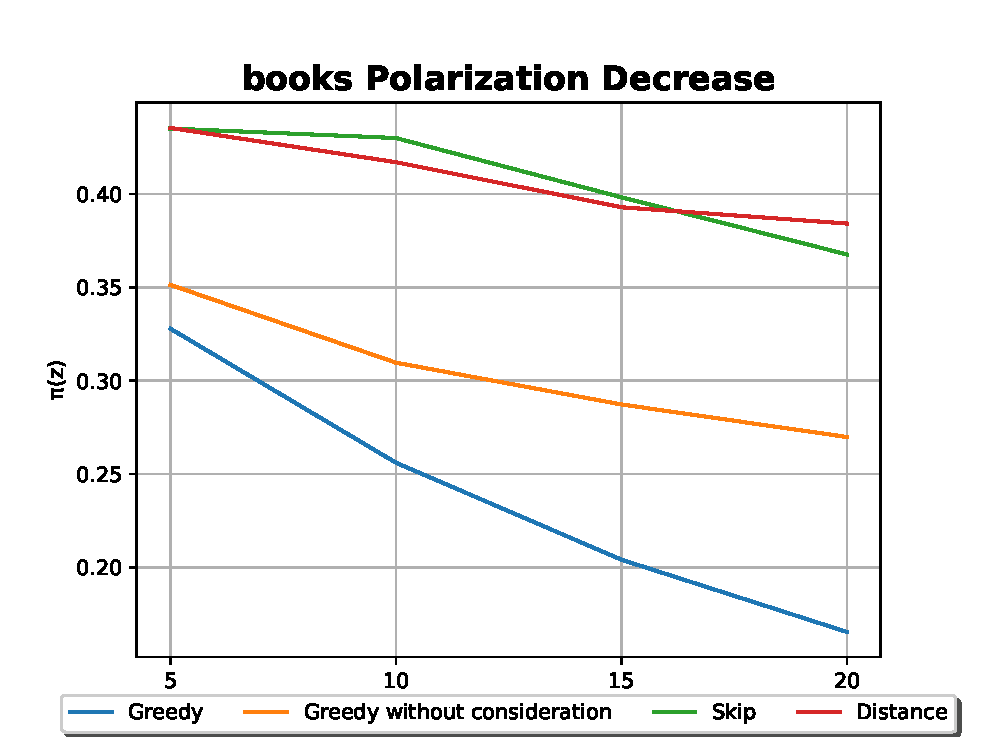
\includegraphics[width=0.65\textwidth]{Figures/books_pol}
	\caption{Heuristic comparison of the decrease}
	\label{fig:books_pol}
\end{figure}


\begin{figure}[!htbp]
	\centering
	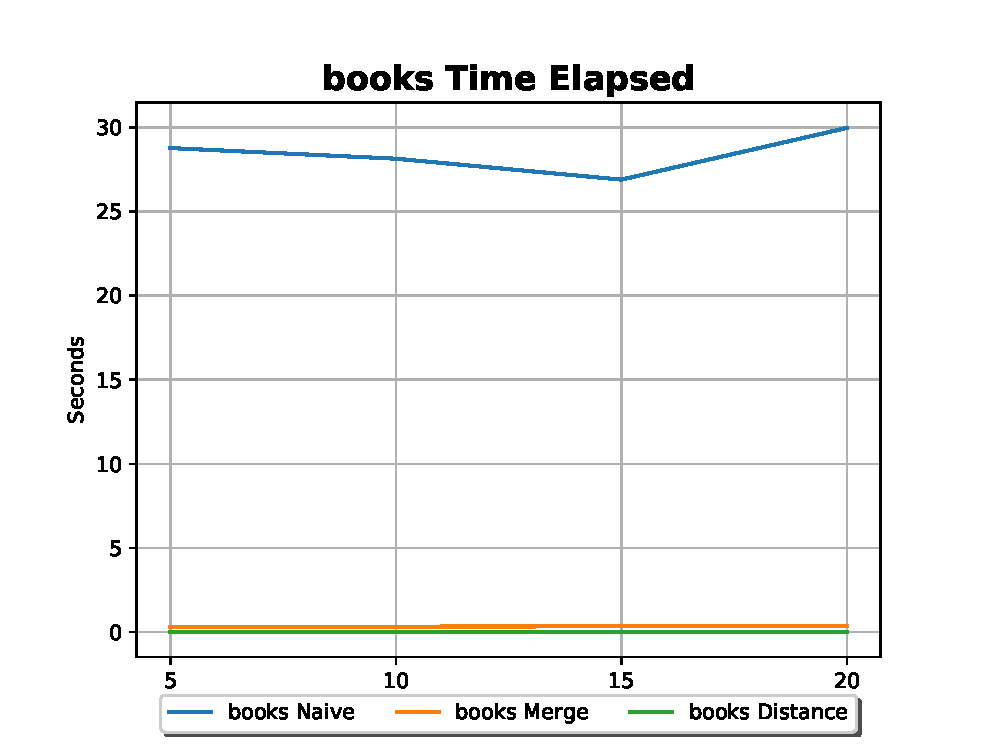
\includegraphics[width=0.65\textwidth]{Figures/books_time}
	\caption{Heuristic comparison of time}
	\label{fig:books_time}
\end{figure}



\section{Polarization in a complete graph}
\label{sec:fullgraph}
\vspace{20pt}
Given a polarized graph $G$ we will compute the polarization index $\pi(z)$ before and after converting the graph $G$ to a full graph. 

\begin{table}[!htbp]
 \centering
 \caption{Polarization Before and after converting to a full graph}
 \label{tab:fullgraph}
 \begin{tabular}{| l || l | l | l | l |}
 \hline
  Dataset & Number of Nodes & Number of edges & Average Degree & $\pi(z)$\\
  \hline
  \hline
  Karate Before & $34$ & $78$ & $4.5882$ &  $0.35857$\\
  \hline
  Karate After & $34$ & $561$ & $33$ &  $0.00081$\\
  \hline
  \hline
  Books Before & $105$ & $441$ & $8.4000$ &  $0.44046$\\
  \hline
  Books After & $105$ & $5460$ & $104.0000$ &  $0.00453$\\
  \hline
  \hline
  Blogs Before & $1490$ & $16718$ & $22.4403$ &  $0.27909$\\
  \hline
  Blogs After & $1490$ & $1109308$ & $1489.0040$ &  $0.00030$\\
  \hline
 \end{tabular}
 \end{table}

\vspace{20pt}
We can see the results from the karate, books and blogs datasets at table ~\ref{tab:fullgraph} The results leads us to the following lemma.
\\	
\begin{lemma}
The polarization index does not drop to zero in a fully connected graph.
\end{lemma}



\section{Experiment by removing edges}
\label{sec:properties}
Bellow we examine the removal of edges from a social graph and their result in polarization. We also use the edge betweenness centrality. The edge betweenness centrality is defined as the number of the shortest paths that go through an edge in a graph or network.(add cite Girvan and Newman 2002). 

In the tables following Sign and Addition refer to the multiplication and the addition of the opinions of the nodes that are attached to the specific edge examined. 
\\

\begin{table}[htbp]
 \centering
 \caption{Edges with the 5 largest decrease (Karate Dataset)}
 \label{tab:edgesLargest}
 \begin{tabular}{| l || l | l | l | l |}
 \hline
  Edge & Betweeness Centrality & Polarization Decrease & Sign & Addition\\
  \hline
  \hline
  (1, 32) & $0.12725$ & $0.04669$ & - &  0\\
  \hline
  (20, 34) & $0.059384$ & $0.03470$ & - &  0\\
  \hline
  (14, 34) & $0.06782$ & $0.02924$ & - &  0\\
  \hline
  (2, 31) & $0.03228$ & $0.02505$ & - &  0\\
  \hline
  (3, 28) & $0.04119$ & $0.02068$ & - &  0\\
  \hline
 \end{tabular}
  
 \caption{Edges with the 5 smallest decrease (Karate Dataset)}
 \label{tab:edgesLargest}
 \begin{tabular}{| l || l | l | l | l |}
 \hline
  Edge & Betweeness Centrality & Polarization Decrease & Sign & Addition\\
  \hline
  \hline
  (6, 7) & $0.00297$ & $0.0$ & + &  -2\\
  \hline
  (5, 11) & $0.00297$ & $5.55111*10^{-17}$ & + &  -2\\
  \hline
  (4, 8) & $0.00336$ & $3.04869*10^{-7}$ & + &  -2\\
  \hline
  (1, 4) & $0.02049$ & $1.38023*10^{-5}$ & + &  -2\\
  \hline
  (32, 34) & $0.05339$ & $1.61826*10^{-5}$ & - &  +2\\
  \hline
  \hline
 \end{tabular}
 
\end{table}

\begin{table}[htbp]
 \centering
 \caption{Edges with the 5 largest decrease (Blogs Dataset)}
 \label{tab:edgesLargest}
 \begin{tabular}{| l || l | l | l | l |}
 \hline
  Edge & Betweenness Centrality & Polarization Decrease & Sign & Addition\\
  \hline
  \hline
  (213, 793) & $0.00219$ & $0.00091$ & - &  0\\
  \hline
  (600, 1183) & $0.00439$ & $0.00074$ & - &  0\\
  \hline
  (523, 1375) & $0.00110$ & $0.00070$ & - &  0\\
  \hline
  (325, 1159) & $0.00110$ & $0.00069$ & - &  0\\
  \hline
  (632, 1000) & $0.00110$ & $0.00069$ & - &  0\\
  \hline
 \end{tabular}
 
 
 \caption{Edges with the 5 smallest decrease (Blogs Dataset)}
 \label{tab:edgesLargest}
 \begin{tabular}{| l || l | l | l | l |}
 \hline
  Edge & Betweenness Centrality & Polarization Decrease & Sign & Addition\\
  \hline
  \hline
  (384, 385) & $9.01465*10^{-7}$ & $0.0$ & + &  -2\\
  \hline
  (301, 644) & $2.11840*10^{-5}$ & $4.64017*10^{-13}$ & + &  -2\\
  \hline
  (775, 1369) & $4.23796*10^{-5}$ & $8.28614*10^{-13}$ & + &  -2\\
  \hline
  (233, 736) & $1.37432*10^{-5}$ & $1.26054*10^{-12}$ & + &  -2\\
  \hline
  (1330, 1410) & $4.08651*10^{-5}$ & $2.12324*10^{-12}$ & + &  +2\\
  \hline
  \hline
 \end{tabular}
 
\end{table}



\begin{table}[htbp]
 \centering
 \caption{Edges with the 5 largest decrease (Books Dataset)}
 \label{tab:edgesLargest}
 \begin{tabular}{| l || l | l | l | l |}
 \hline
  Edge & Betweeness Centrality & Polarization Decrease & Sign & Addition\\
  \hline
  \hline
  (53, 76) & $0.06290$ & $0.01985$ & - &  0\\
  \hline
  (46, 102) & $0.04914$ & $0.01541$ & + &  -2\\
  \hline
  (19, 77) & $0.04367$ & $0.01458$ & + &  +2\\
  \hline
  (9, 51) & $0.02812$ & $0.01000$ & - &  0\\
  \hline
  (49, 72) & $0.06809$ & $0.00952$ & - &  0\\
  \hline
 \end{tabular}
 
 
 \caption{Edges with the 5 smallest decrease (Books Dataset)}
 \label{tab:edgesLargest}
 \begin{tabular}{| l || l | l | l | l |}
 \hline
  Edge & Betweeness Centrality & Polarization Decrease & Sign & Addition\\
  \hline
  \hline
  (13, 40) & $0.00305$ & $3.89807*10^{-9}$ & + &  +2\\
  \hline
  (35, 37) & $0.00078$ & $8.65544*10^{-9}$ & + &  +2\\
  \hline
  (88, 89) & $0.00036$ & $1.00835*10^{-8}$ & + &  -2\\
  \hline
  (65, 69) & $0.00072$ & $1.51261*10^{-8}$ & + &  -2\\
  \hline
  (35, 36) & $0.00146$ & $2.92727*10^{-8}$ & + &  +2\\
  \hline
  \hline
 \end{tabular}
 
\end{table}


We can clearly see that there is not a direct association between the edge betweenness centrality and the decrease in polarization. For example in the karate dataset edge (20,34) has almost the same betweenness centrality with edge (32,34). The first is among the edges that their removal contributes in one of the biggest polarization decreases while the other is among the ones with the smallest. A second thing that we can see in all three datasets is that the biggest decrease is coming from the removal of edges that connect opposing opinions.
